\section{同调群的拓扑不变性}
\sourcepage{117--118}
本节实现本章的主要目标：证明单纯同调群的拓扑不变性。

\entry{定义}{2.6.1}设 $K,L$ 为单纯复形，$h:|K|\to|L|$ 连续。选择 $K$ 的剖分 $K'$，使 $h$ 有单纯逼近 $f:K'\to L$。令 $\lambda:\mathcal C(K)\to\mathcal C(K')$ 为剖分算子。定义\textbf{由 $h$ 诱导的同态}
\[
h_*:H_p(K)\to H_p(L),\qquad h_*=f_*\circ\lambda_*.
\]
一旦选定 $K'$，此同态就不依赖于具体逼近 $f$，因为任意两个逼近都邻接。

若 $g:K'\to K$ 为恒等映射的单纯逼近，则 $\lambda_*,g_*$ 互逆，所以也可定义 $h_*=f_*\circ g_*^{-1}$。利用这一点，证明它与剖分选择无关。设 $K''$ 为另一个允许单纯逼近的剖分。

先考虑容易的情形：恒等映射有单纯逼近 $k:K''\to K'$，于是有单纯映射
\[
K''\xrightarrow{k}K'\xrightarrow{g}K,\qquad K'\xrightarrow{f}L.
\]
则 $gk,fk$ 分别为恒等映射和 $h$ 的单纯逼近，使用 $K''$ 定义的同态为
\[
(fk)_*\circ(gk)_*^{-1}=(f_*k_*)\circ(g_*k_*)^{-1}=f_*g_*^{-1},
\]
与使用 $K'$ 相同。

一般地，选择 $K$ 的剖分 $K'''$，使恒等映射有单纯逼近 $k_1:K'''\to K'$ 和 $k_2:K'''\to K''$。使用 $K'''$ 得到的同态，与使用 $K'$ 或 $K''$ 相同，故定义良好。

应说明，$h_*$ 不仅依赖于空间 $X=|K|$、$Y=|L|$ 和映射 $h:X\to Y$，还依赖于以它们为多胞体的具体复形。若 $M,N$ 也是 $X,Y$ 的复形，$h$ 也诱导 $H_p(M)\to H_p(N)$。严格来说应以 $(h_{K,L})_*$ 或 $(h_{M,N})_*$ 区分。这里仍用简单记号 $h_*$，由上下文说明。定义可三角剖分空间的同调时将在第 3.6 节进一步讨论。

\entry{定理}{2.6.2（函子性质）}恒等映射 $i:|K|\to|K|$ 诱导恒等同态 $i_*:H_p(K)\to H_p(K)$。若 $h:|K|\to|L|$、$k:|L|\to|M|$ 连续，则 $(k\circ h)_*=k_*\circ h_*$。约化同调也有相同结论。

\noindent\textbf{证明：}第一条立即由定义得到。为证第二条，选择 $f_0:L'\to M$、$g_0:L'\to L$ 分别逼近 $k$ 和 $|L|$ 的恒等映射；再选择 $f_1:K'\to L'$、$g_1:K'\to K$ 分别逼近 $h$ 和 $|K|$ 的恒等映射。

\sourcepage{119--120}
$f_0f_1$ 是 $kh$ 的单纯逼近，故
\[
(kh)_*=(f_0f_1)_*(g_1)_*^{-1}.
\]
$g_0f_1$ 是 $h$ 的单纯逼近，故
\[
h_*=(g_0f_1)_*(g_1)_*^{-1},\qquad k_*=(f_0)_*(g_0)_*^{-1}.
\]
综合等式并用定理 1.13.3，得到 $(kh)_*=k_*h_*$。\hfill$\square$

\entry{推论}{2.6.3（同调群的拓扑不变性）}若 $h:|K|\to|L|$ 为同胚，则 $h_*:H_p(K)\to H_p(L)$ 为同构。约化同调也如此。

\noindent\textbf{证明：}取逆映射 $k$，则 $h_*k_*=(i_{|L|})_*$，$k_*h_*=(i_{|K|})_*$，均为恒等映射。因此 $h_*$ 为同构。\hfill$\square$

\subsection*{在相对同调中的应用}
以上证明了绝对同调群的拓扑不变性。对相对同调，把复形换为复形与子复形组成的偶，应用定理 1.13.11、引理 2.2.7 与定理 2.5.5，所有论证原样成立。将结果重述如下。

\entry{定理}{2.6.4}
\begin{enumerate}[label=(\alph*)]
\item $(|K|,|K_0|)$ 的恒等映射诱导相对同调的恒等同态。
\item 若连续映射为 $(|K|,|K_0|)\xrightarrow{h}(|L|,|L_0|)\xrightarrow{k}(|M|,|M_0|)$，则相对同调中 $(kh)_*=k_*h_*$。
\item 若同胚 $h:|K|\to|L|$ 将 $|K_0|$ 映到 $|L_0|$ 上，则 $h_*$ 是相对同调同构。
\end{enumerate}
下面单独定义经常使用的收缩映射概念，习题围绕它展开。下一节的定义 2.7.10 将加强此概念。

\entry{定义}{2.6.5}若 $A\subset X$，则\textbf{收缩映射}（retraction）$r:X\to A$ 是满足对所有 $a\in A$ 有 $r(a)=a$ 的连续映射。若存在这样的映射，称 $A$ 为 $X$ 的\textbf{收缩核}（retract）。

\subsection*{习题}
\begin{enumerate}
\item \begin{enumerate}[label=(\alph*)]
\item 若 $r:X\to A$ 为收缩映射，$X$ 为 Hausdorff 空间，证明 $A$ 在 $X$ 中闭。
\item 若 $K_0$ 为 $K$ 的子复形，$r:|K|\to|K_0|$ 为收缩映射，证明 $r_*:H_p(K)\to H_p(K_0)$ 满射，而包含映射 $j$ 诱导的 $j_*$ 单射。
\item 证明不存在收缩映射 $r:B^n\to S^{n-1}$。
\end{enumerate}
\item \begin{enumerate}[label=(\alph*)]
\item 证明存在从 Klein 瓶 $S$ 到图 2.6.1 中嵌入圆周 $A$ 的收缩映射，但不存在到圆周 $C$ 的收缩映射。
\item 证明不存在从射影平面到图 2.6.2 中嵌入圆周 $C$ 的收缩映射。
\end{enumerate}
\begin{center}
\begin{minipage}{.47\textwidth}\centering
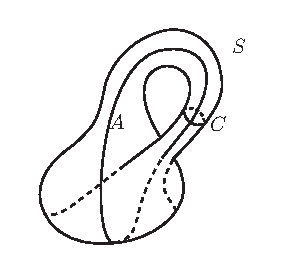
\includegraphics[width=52mm]{figures/2-6-1.pdf}\\图 2.6.1
\end{minipage}\hfill
\begin{minipage}{.47\textwidth}\centering
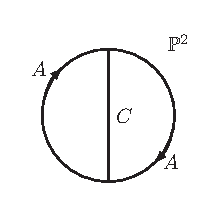
\includegraphics[width=41mm]{figures/2-6-2.pdf}\\图 2.6.2
\end{minipage}
\end{center}
\item 判定是否存在从环面到图 2.6.3 中管状区域 $A$、圆盘 $B$、圆周 $C$ 的收缩映射。
\begin{center}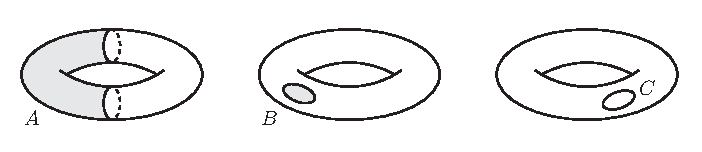
\includegraphics[width=122mm]{figures/2-6-3.pdf}\\图 2.6.3\end{center}
\item 确定所有存在从圆周 $C$ 到它的收缩映射的空间 $X$。
\end{enumerate}
